%---------------------------------------------------------------
%	PACKAGES AND OTHER DOCUMENT CONFIGURATIONS
%--------------------------------------------------------------
\documentclass[paper=a4, french, 11pt]{scrartcl} 

\usepackage[utf8]{inputenc} 
\usepackage[T1]{fontenc} % Use 8-bit encoding that has 256 glyphs
\usepackage{fourier} 
\usepackage[francais]{babel} % English language/hyphenation
\usepackage{amsmath,amsfonts,amsthm} % Math packages
\usepackage{colortbl}
\usepackage{graphicx}
\usepackage{sectsty} % Allows customizing section commands
\usepackage{fancyhdr} % Custom headers and footers


\allsectionsfont{\centering \normalfont\scshape} 

\sectionfont{\normalfont\scshape}
\subsectionfont{\normalfont\scshape}
\subsubsectionfont{\normalfont\scshape}

\pagestyle{fancyplain} 
\fancyhead{} 
\fancyfoot[L]{} % Empty left footer
\fancyfoot[C]{} % Empty center footer
\fancyfoot[R]{\thepage} % Page numbering for right footer
\renewcommand{\headrulewidth}{0pt} % Remove header underlines
\renewcommand{\footrulewidth}{0pt} % Remove footer underlines

\setlength{\headheight}{13.6pt} % Customize the height of the header
\setlength\parindent{0pt} 

\definecolor{bg}{RGB}{235,235,235}
\definecolor{bk}{RGB}{135,135,135}
\newcommand{\class}[1]{\colorbox{bg}
{\textcolor{red}{\usefont{OT1}{cmtt}{m}{n}#1}}}
\newcommand{\cmd}[1]{\colorbox{bk}{\textcolor{white}
{\usefont{OT1}{cmtt}{m}{n}#1}}}
\newcommand{\horrule}[1]{\rule{\linewidth}{#1}}

%-----------------------------------------------------------
%	TITLE SECTION
%-----------------------------------------------------------

\title{	
\normalfont \normalsize 
\textsc{Projet INF582} \\ [25pt] 
\horrule{0.5pt} \\[0.5cm] % Thin top horizontal rule
\huge Text detection \\ % The assignment title
\horrule{2pt} \\[0.5cm] % Thick bottom horizontal rule
}

\author{Zhixing CAO, Yuesong SHEN} % Your name

\date{\normalsize\today} % Today's date or a custom date

\begin{document}

\setlength\parindent{12pt}
\maketitle % Print the title

\section{Introduction}
The development of smartphones and the growing demands in content-based image understanding has made the text detection a crucial topic in machine-human interaction. It has been shown that the performance of image retrieval depends critically on the performance of text detection and recognition. For example, two book covers with different titles but identical background prove to be considered virtually indistinguish without detecting and recognizing the text.

\subsection{Goal of project}
Early approach of text detection and recognition techniques such as OCR can be traced in early 1900s. Recent years, with the progress in the field of machine learning pattern recognition and text localisation techniques make new breakthroughs. With the study of some of those techniques, our project concern algorithms that can decode the text in images.

The approach of our project can be divided into two parts --- text detection and text recognition. The detection part detect potentiel texts in images and output pure text candidates and the recognition part translate the image of text candidates to digital texts that can be read by machines.

\subsection{Work breakdown}
The whole project is carried out by Zhixing CAO and Yuesong SHEN. Several works have been carried out independently during the project. Here is the overview of work breakdown.\
\begin{figure}[h]
\begin{center}
	\vspace{-3ex}
   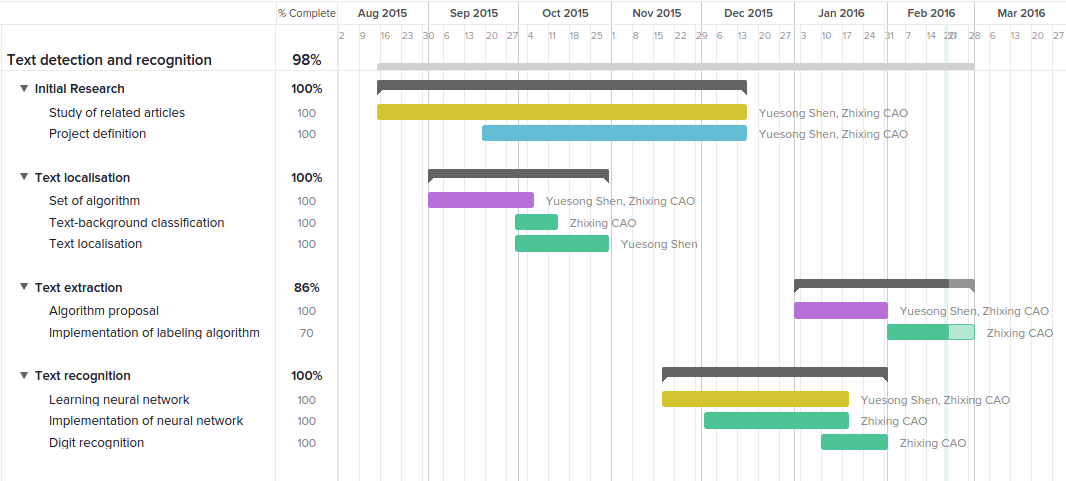
\includegraphics[width=0.9\linewidth]{breakdowns.png}
\end{center}
\vspace{-4ex}
\caption{Work breakdown}
\label{fig:heatmap}
\end{figure}
 
\section{State of the art}
\subsection{Text detection}
As an essential prerequiste for text recognization, text within images has to be robustly located. This is challenge task due to the variety of the text form, such as variations in languages, font and style, geometric and photometric distortions, partial occlusion, and lightening conditions. Text detection problem has been studied a lot in recent researches and numerous methods are reported in the literature.

All the methods used in recent research can be classified into two catagories: method based on texture and method based on connected componet.

Texture-based method views texts as a special texture that is distinguishable from its background. Features are extracted over some special regions and a classifier is used to identify texts areas. Zhong and al have segmented caption text regions from background and used the intensity variation information. Ye and al have proposed a method using multiscale wavelet features and a coarse-to-fine algorithm to locate text lines under different backgrounds.

Different with the texture-based method, the connected component based approach extracts regions from the image and selects text candidates using some geometric rules. In ICDAR 2005 text locating competition, the best result applies have used an adaptive binarization method to find connected components and forms text lines based on geometric properties. Recently Chen and al extract letter candidates by employing edge-enhanced Maximally Stable Extremal Regions and using geometric and stroke width information to exclude non-text objects. They have achieved an accuracy score of 95\%.

\subsection{Text recognition}
Converting text data from image and deciphering into digits is an important problem. Early physical photocell-based OCR implemented matrix matching by comparing an image to a stored glyph on a pixel-by-pixel basis. Those algorithms involve mostly extensive processing on the image such as thinning, smoothing contour analysis etc. because the majority of previous works uses geometrical and topological features. In recent research community the dominant approach to this problem is based on machine learning techniques --- a general inductive process building automatically a classifier by learning.

In the textbook \textit{Pattern Recognition and Machine Learning}, Bishop reflects recent developments in the field of pattern recognition and machine learning and shows potential usages of machine learning method in pattern recognition. The early effort has been made around 1986s by Burr, Mehr\&Richfield to implement a neural network in character recognition. Recently, with the development of parallel computation and the use of GPU, efficient OCR system based on neural network is realized. 

\subsection{Our approach}
In this report, we show you our approach of the text detection problem by combined texture-based method and connected component based method and our text recognition algorithm using neural network. 

We adapte at first the method proposed by Liu and al to locate texts. This algorithm detects text candidate by applied classifier on contour pictures of the original image. Experimental results demonstrate that this approach is robust for varied font-size, font-color, background and languages, which can be used efficiently.

After locating the text, a connected component based method is used to extract word candidates. We find all components by using connected-component labeling algorithm. Then we use some geometric constraints and heuristic rules to merge them and extract letters and words candidates.  

Our approach for text recognition is based on using neural network to classify characters. With a training set of different kind of characters, the neural network is constructed in order to match an input character to a learned one. 

\section{Text detection}
In order to extract text from an image, we first need to determine the location of text zone in order to later perform the text recognition.  
\subsection{Detecton of contour}
Since text is always composed of strokes (so that it can be written by men), edge turns out to be an excelent characteristic for text zone identification. We have adopted the approach proposed by Liu and al. for edge information extraction, that is by applying Sobel edge detector on the image for 4 directions (vertical, horizontal, up-right to down-left and up-left to down-right) with distance defined on the RGB color space to get 4 edge maps. And this 4 edge maps are to be used to determine the text locations.

\begin{figure}[h]
\begin{center}
	\vspace{-3ex}
   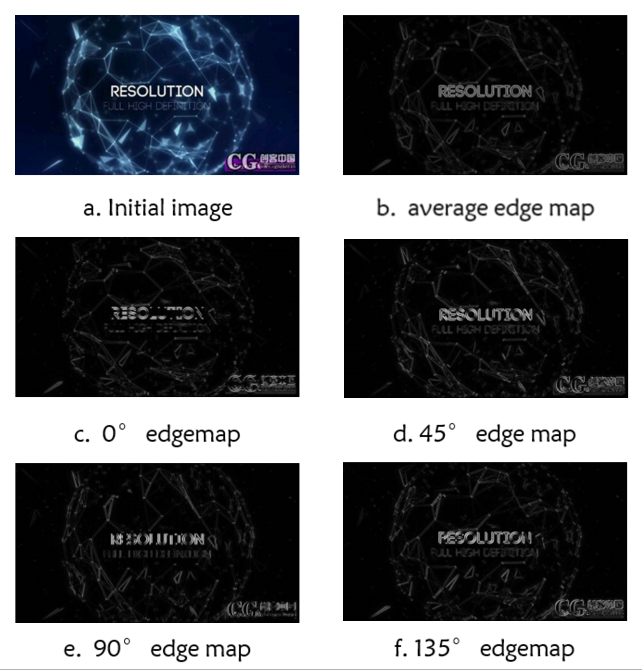
\includegraphics[width=0.75\linewidth]{edge_filter_example.png}
\end{center}
\vspace{-4ex}
\caption{Edge maps}
\label{fig:heatmap}
\end{figure}

\subsection{K-means classification}
With the 4 edge maps, we can then apply a sliding window of size $w \times h$ to calculate the 6 different features as follows:

$\mu = \frac{1}{w \times h} \sum_{i=1}^{w} \sum_{j=1}^{h} E(i,j)$

$\sigma =\sqrt{\frac{1}{w \times h} \sum_{i=1}^{w} \sum_{j=1}^{h} (E(i,j) - \mu)}$

$Et = \sum_{i,j} E(i,j)\dot \log E(i,j) $

$I = \sum_{i,j} (i-j)^2 E(i,j)$

$H = \sum_{i,j} \frac{1}{1+(i-j)^2}E(i,j)$

Where $E(i,j)$ is the value of pixel in i\textsuperscript{th} row, j\textsuperscript{th} column, here it is the grayscale color of a pixel in an edge map. $\mu$ is the mean value in sliding window, $\sigma$ is their standard deviation, $ Et$ is their entropy, $ I$  is their gravity center and $ H$ is the expectation.

With the 4 edge maps, we then get 24 features for a given position of the sliding window. And since there is no apparent cost function available, we need an unsupervised clustering algorithm to distinguish text zones from their surroundings. We apply therefore the k-means algorithm for this, as proposed in the paper of Liu and al.

This approach, while effective for seperatings text and non-text zones, can not determine which one of the 2 zones is text zone, due to its non-supervised nature. We therefore need some extra effort to choose the text zone. There is no solution proposed in the original article. We propose 2 ideas to solve this problem: The first approach is to collect a set of manually choosed text and non-text data (an average feature vector for each zone in each image) and then train a classifier with supervised learing approach. The second approach is to use geometrical and topological informations of each zone to determine text zones.

\subsection{Text area identification}
The result obtained by k-means algoritm needs to be polished to remove noise and other non text zone. We first use morphology operations “open” and “dilate” to fill up tiny holes and gaps and remove too small zones in the background. We can then apply some empirical rules to further remove zones which can not contain text. Each connected component of the refined text zones will then be boxed by a rectangle and returned as final results.

\begin{figure}[h]
\begin{center}
	\vspace{-3ex}
   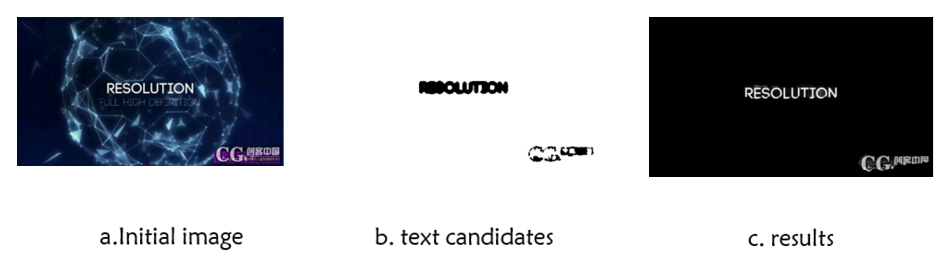
\includegraphics[width=0.9\linewidth]{text_area_example.png}
\end{center}
\vspace{-4ex}
\caption{Text area identification}
\label{fig:heatmap}
\end{figure}

\subsection{Connected components detection}
The former method shows efficient results. However, it is still incapable of distinguishing each character which is important for text recognition. So we use at next step the connected connected components algorithm to extract characters.

At first, we set the input image into a binary matrix according to a threshold. Knowing that all colors can be encoded into a grayscale double number between 0 and 255, we can transform our input image by setting all pixels to 0 or 1 with their grayscale number by a threshold. Most of the time, pixels in a single letter have similar colors, so that in the binary matrix, these pixels have always the same value which will be considered as a same component.

The connected-component labeling algorithm is based on union-find method. The first pass of the algorithm propagate a pixel's label to its eight neighbors. Whenever the situation of connectivity arises, we attribute labels and union two set if it's neccesary. At the end of the first pass, each equivalence class has been completely determined and has a unique label, which is the root of its tree in the union-find structure. A second pass through the image then performs a translation, assigning to each pixel the label of its equivalence class.

\begin{figure}[h]
\begin{center}
	\vspace{-3ex}
   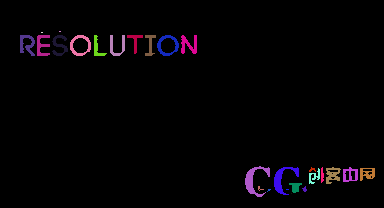
\includegraphics[width=0.75\linewidth]{connected_components_example.png}
\end{center}
\vspace{-4ex}
\caption{Connected components detection}
\label{fig:heatmap}
\end{figure}

\subsection{detection of words}

In many language, a single character can be composed by several different part. So after the connected component detection, we calculate the gravity center of each component and attribute those who have nearby center coordinates component a common label.  

\section{Text recognition}
\subsection{Neural network}
After extract characters, we can move to the next step and try to recognize them.

In machine learning, neural network is a powerful tool to estimate functions that maps input to output. Theoretically, it can approximate every non-linear functions when using a non-linear activation function. 

Inspired of humans' central nervous systems, neural network uses connected nodes, known as neurons, to imitate the nervous system. A neural network is a complex adaptive system with ability to \textit{learn}. It consists of multiple layers. Apart from the input layer, all layers have an activation function. By adjusting this function according to our given datas, known as training set, the network achieve to learn and understand these datas. Here is the structure of the neural network:

\begin{figure}[h]
\begin{center}
	\vspace{-3ex}
   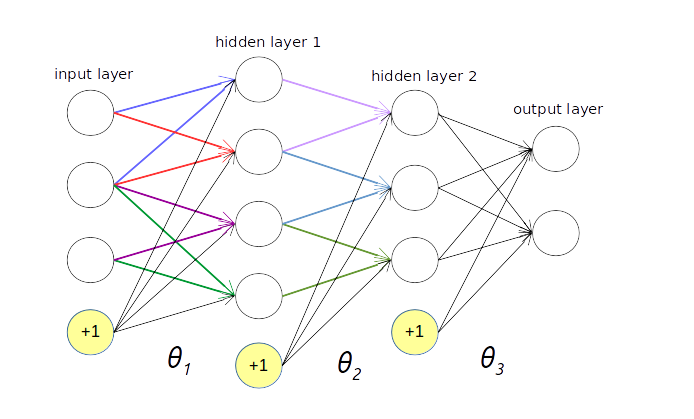
\includegraphics[width=0.75\linewidth]{network.png}
\end{center}
\vspace{-4ex}
\caption{Structure of neural network}
\label{fig:heatmap}
\end{figure}

Our goal is to determine the activation function $\Theta$ by using gradient descent. At first, we need to initialize $\Theta$ by some random values in order to break the symmetry. Then, the forward propagation will determine the output while the backpropagation will correct the error.

In our project, we use neural network to learn digital numbers.

\subsection{Pattern recognition}
In essence, pattern recognition convers the following problem: 'Given examples of signals and the correct decisions of them, make decisions automatically with future streams'. In our project, we use the neural network to learn a set of examples of digital numbers' images. Then we use the same neural network to predict new digital numbers' images. 

\section{Result}
\subsection{Text detection}
\subsection{Text recognition}
We use the MNIST database which consists of digits written by high school students and employees of the United States Census Bureau as our training data. The MNIST dataset consists of 70.000 handwritten digit images of 0 to 9.

We have tested the network with 10.000 different images and with different parameters of the network.

\subsubsection{Influence of different parameters}
~\indent
Here are some results with different parameters:

\begin{small}
	\begin{tabular}{ |c|c|c|c|c| }
	\hline
	$num\_training\_data$ & $num\_layers$ & $num\_nodes$ & $num\_iteration$ & $accuracy$ \\
	\hline
	60000 & 1 & 200  & 30 & 92.56 \\
	\hline
	6000 & 1 & 200  & 30 & 91.96 \\
	\hline
	6000 & 1 & 20  & 30 & 91.02 \\
	\hline
	6000	 & 1 & 10  & 30 & 84.59 \\
	\hline
	6000 & 2 & 20,20  & 30 & 85.7\\
	\hline
	6000 & 2 & 20,20  & 45 & 90.33\\
	\hline
	\end{tabular}
\end{small}

We notice that we can get fairly good result by well choosing the parameters of the neural network such as the number of layers, number of nodes, size of training data etc.. 

\subsubsection{Confusion matrix}
In order to better visualize the performance of the algorithm, we use here the confusion matrix to see if the system is confusing two classes. Here is the heatmap of the confusion matrix:

\begin{figure}[h]
\vspace{-1ex}
\begin{center}
   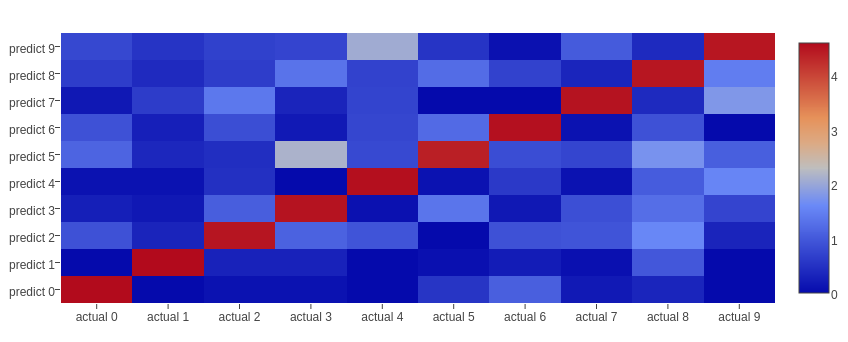
\includegraphics[width=1.0\linewidth]{heatmap_log.png}
\end{center}
\vspace{-3ex}
\caption{Heatmap of confusion matrix}
\label{fig:heatmap}
\end{figure}

Each color corresponds with $log\frac{number\_of\_predicted\_i}{number\_actual\_ i}$, with this map, we can easily determine the error caused by the confusion of numbers. For exemple, the wrong prediction of number 3 is always 5 and the wrong prediction of number 4 is always 9. That is to say, the hand-writting of 4 is similary to the hand-writting of 9 and sometimes, it may lead to confusion in our system.




\end{document}